\documentclass[glossy]{beamer}
\useoutertheme{wuerzburg}
\useinnertheme[realshadow,corners=2pt,padding=2pt]{chamfered}
\usecolortheme{shark}

\usepackage{listings}
\usepackage[utf8]{inputenc}

\usepackage{tikz}
\newcommand<>{\hover}[1]{\uncover#2{%
 \begin{tikzpicture}[remember picture,overlay]%
 \draw[fill,opacity=0.4] (current page.south west)
 rectangle (current page.north east);
 \node at (current page.center) {#1};
 \end{tikzpicture}}
}

\title{Arquitecturas y Organización de Computadoras I\\\line(1,0){320}}
% \author{\texorpdfstring{Author\newline\url{email@email.com}}{Author}}
%\author{Rafael Ignacio Zurita}
\institute{Rafael Ignacio Zurita \\ Departamento de Ingenieria de Computadoras - FAI - UNCOMA 2018 \\ Clase presencial 6b}
%\date{\today}



\begin{document}




\begin{frame}
\maketitle
\end{frame}

\institute{Rafael Zurita - Departamento de Ingenieria de Computadoras - FAI - UNCOMA \\ 2018}





\begin{frame}
\frametitle{Máquinas Algoritmicas}
\textbf{UNIDAD 2: Máquinas algorítmicas}

\begin{enumerate}
\item Máquinas algorítmicas de propósito específico
\begin{itemize}
\item Algoritmos de multiplicación
\begin{itemize}
\item Simple, para números sin signo
\item Algoritmo de Booth,  para números con signo
\end{itemize}
\end{itemize}
\item Máquinas algorítmicas de propósito general
\begin{itemize}
Procesador (CPU)
\end{itemize}

\end{enumerate}
\end{frame}


\begin{frame}
\frametitle{Máquinas Algoritmicas}
\textbf{UNIDAD 2: Máquinas algorítmicas}

Una máquina algorítmica consiste en un sistema digital capaz de materializar  y 
ejecutar un determinado algoritmo

\begin{enumerate}
\item Máquinas algorítmicas de propósito específico: Algoritmos de multiplicación
\begin{itemize}
\item Más complicada que la suma
\item Se realiza con desplazamientos y sumas.
\item Más tiempo y más superficie.
\item Veremos algoritmos sencillos para números positivos 
\end{itemize}
\end{enumerate}

\end{frame}




\begin{frame}
\frametitle{Máquinas Algoritmicas}

\begin{center}
\begin{figure}
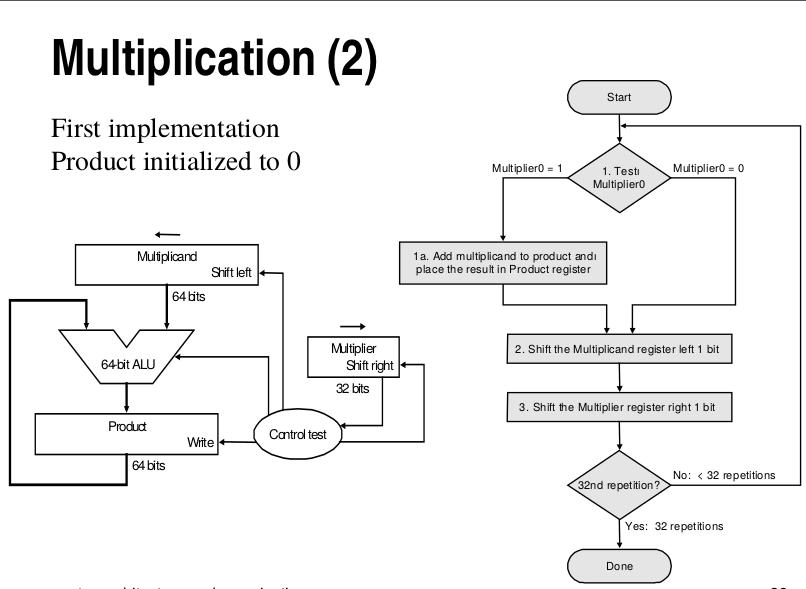
\includegraphics[scale=0.4]{mult1.jpg} 
\end{figure}
\end{center}
\end{frame}



\begin{frame}
\frametitle{Máquinas Algoritmicas}

\begin{center}
\begin{figure}
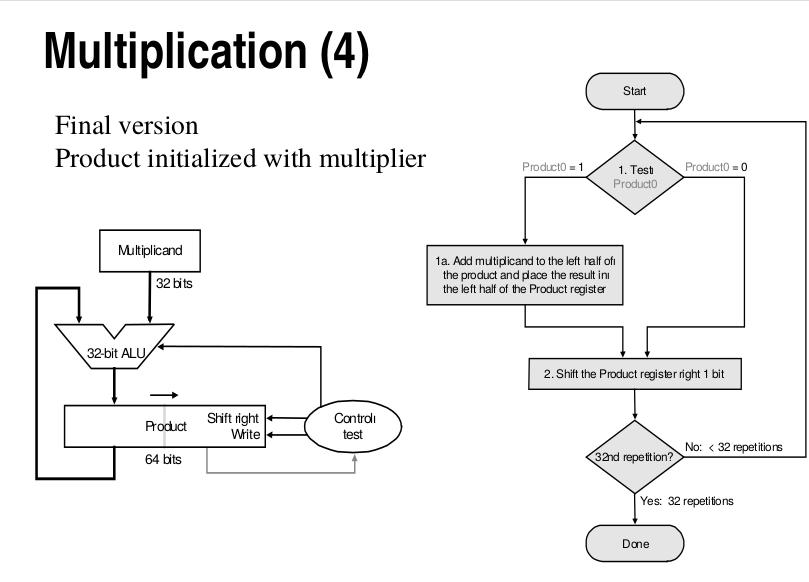
\includegraphics[scale=0.4]{mult2.jpg} 
\end{figure}
\end{center}
\end{frame}





\begin{frame}
\frametitle{Máquinas Algoritmicas}
\begin{center}
\begin{itemize}
\item  ¿Preguntas?
\item  Próxima clase: Máquina Algoritmica de propósito general: CPU
\end{itemize}
\end{center}
\end{frame}





\begin{frame}
 \frametitle{Bibliografía}
        \begin{center}
        \textbf{Material complementario de estudio}
        \end{center}
Libros
\begin{itemize}
\item Andrew S. Tanenbaum (2000), ORGANIZACIÓN DE COMPUTADORAS un enfoque estructurado, Editorial Prentice Hall. (10 copias en biblioteca)
\item David. Patterson John L. Hennessy (1995), ORGANIZACIÓN Y DISEÑO DE COMPUTADORES La interfaz hardware/software, McGraw-Hill (8 copias en biblioteca).
\end{itemize}

\end{frame}


\end{document}
